\documentclass[11pt,a4paper]{article}
% Generated from new_paper/paper.md by scripts/build/build_latex.py -- edit the markdown, not this file.
\usepackage[utf8]{inputenc}
\usepackage[T1]{fontenc}
\usepackage{lmodern}
\usepackage[margin=2.5cm]{geometry}
\usepackage{amsmath}
\usepackage{graphicx}
\usepackage{microtype}
\usepackage[hidelinks]{hyperref}
\usepackage{setspace}
\usepackage{lineno}
\usepackage{caption}
\captionsetup{labelformat=empty,skip=2pt}
\setlength{\parskip}{6pt}
\setlength{\parindent}{0pt}
\date{}
\onehalfspacing
\linenumbers
\begin{document}
\title{Supplementary Information}
\maketitle

Additional file 1 for: Growth fitness, not drug tolerance, explains most pre-treatment prediction of cancer cell fate

\section*{Supplementary Notes}

\textbf{Supplementary Note 1. Graph model and hyperparameter sweep.} We built a cell--cell k-nearest-neighbour graph within each sample and trained a GraphSAGE-style network (Hamilton et al., 2017). Its encoder was optionally pretrained with a contrastive loss (Chen et al., 2020) that pulls pre-treatment sisters together, excluding test cells. The idea was that sister pairs mark the heritable part of the state, which is what the ceiling analysis says a predictor must use. Across three seeds, sister-pair pretraining improved a matched MLP slightly in every arm (by 0.004--0.014; MLP 0.700--0.738, pretrained MLP 0.708--0.742). Message passing over the graph did not help: the graph network with pretraining reached 0.696--0.734 (seed s.d. $\leq$ 0.005), slightly below the pretrained MLP and below logistic regression (0.708--0.747) in every arm (Fig. S1). In replicate hold-out, the graph network scored 0.68--0.74, against 0.70--0.76 for logistic regression. Smoothing features over the same graph before logistic regression changed AUROC by at most 0.005. A one-at-a-time sweep of the graph network without pretraining over the number of layers, hidden width, dropout, learning rate, weight decay and neighbourhood size (Table S18) gave 0.727--0.739 for carboplatin, 0.722--0.733 for olaparib, 0.695--0.714 for NK and 0.667--0.700 for control, never above logistic regression. The neural models therefore recovered the same signal as the linear model, and no more.

\textbf{Supplementary Note 2. Pre-specified marker panel and the IGF axis.} To check this at the level of individual genes, we fixed a panel of 28 marker genes in advance, covering proliferation, G1 arrest, senescence, quiescence and previously reported persister markers (Fig. S3; 24 were among the retained genes). In the control contrast, recovered cells expressed markedly less of the CDK inhibitors CDKN1A (p21; z = $-$4.8, FDR $<$ 10$^-$$^4$), CDKN1B and CDKN1C, which fits a proliferative fitness state. Beyond the control contrast, the replication and mitosis genes CDK1, PCNA, MCM2 and E2F1 were lower in pre-resistant cells in all three drug arms (z between $-$1.2 and $-$4.3). Individually, however, only CDK1 and PCNA for NK cells passed correction (FDR 0.017 and 0.003). Senescence-associated secretory genes (IL6, CXCL8, SERPINE1) were not higher in pre-resistant cells, and CDKN1C was only modestly and non-significantly higher. The drug-specific state therefore looks like slower cycling among otherwise fit cells rather than senescence, although at the level of single genes the evidence is weak.

Among the drug-specific genes were several members of the insulin-like growth factor axis. IGFBP7 and IGF2BP1 were drug-specific for both carboplatin (FDR 0.002 and 0.015) and olaparib (FDR 0.001 and $<$ 0.001), and IGF2 for olaparib (FDR $<$ 0.001). None was drug-specific for NK cells: IGFBP7 passed the test of difference from the control contrast (FDR 0.039) but not the drug contrast itself, so it is starred in Fig. S3 without being called drug-specific (Table S16), and IGFBP2 itself was not drug-specific in any arm (in the olaparib arm it was differentially expressed, FDR 0.012, but not significantly differently from the control contrast, FDR 0.78). IGF-1 receptor signalling supports drug-tolerant persisters (Sharma et al., 2010), and IGFBP2 confers afatinib tolerance in triple-negative breast cancer (Pellecchia et al., 2024). We note the overlap as a hypothesis, not a finding. CD44, which marked multi-treatment resistance in melanoma (Schaff et al., 2026), was lower, not higher, in pre-resistant cells in all three drug arms (FDR $\leq$ 3 $\times$ 10$^-$$^6$) and was not differentially expressed in the control arm (FDR 0.45). The difference from the control contrast was significant for olaparib and NK cells (FDR 0.006 and 0.007) but not for carboplatin (FDR 0.12). In melanoma, CD44-high cells resisted MAPK inhibitors and hypoxic stress, whereas CD44-low cells were more resistant to doxorubicin (Schaff et al., 2026), so the direction of a pre-existing marker may depend on the kind of stress.

\textbf{Supplementary Note 3. Inferred copy-number subclones.} Dai et al. (2024) reported that InferCNV subclone A was enriched among pre-resistant cells under all treatment conditions, especially carboplatin and olaparib. Its signature was also positively associated with the treatment pre-resistance signatures and negatively with the control pre-survival signature. Per-cell subclone calls are not public, so we inferred copy-number profiles ourselves with infercnvpy (11,883 genes, 970 genomic windows) and clustered them (k = 6, chosen by silhouette). The clusters were only weakly separated (silhouette 0.21). Still, the largest cluster reproduced the published pattern: it was over-represented among pre-resistant cells in the carboplatin (odds ratio 2.24), olaparib (2.04) and NK (1.34) arms (all FDR $<$ 10$^-$$^3$), but not in the control arm (1.14, p = 0.14).

Cluster identity alone predicted the labels poorly (AUROC 0.54--0.60). Within clusters, the expression model kept most of its performance (0.69--0.72), and expression added strongly to a model that already contained cluster identity (likelihood-ratio p $<$ 10$^-$$^5$$^0$ in every arm). Copy-number composition thus accounts for a small, largely treatment-specific part of the labels. It is one plausible source of the drug-specific component, but not of the shared transcriptional signal.

\section*{Supplementary Figures}

\begin{figure}[!htbp]
  \centering
  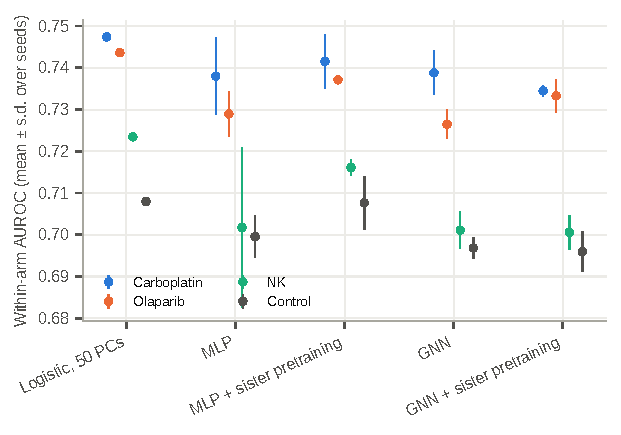
\includegraphics[width=\linewidth]{figures/FigS1_gnn_ablation.pdf}
  \caption*{\textbf{Supplementary Fig. 1 | Graph model ablation.} Within-arm AUROC for logistic regression, an MLP, an MLP with sister-pair pretraining, the graph network, and the graph network with pretraining (mean $\pm$ s.d. over seeds).}
\end{figure}


\begin{figure}[!htbp]
  \centering
  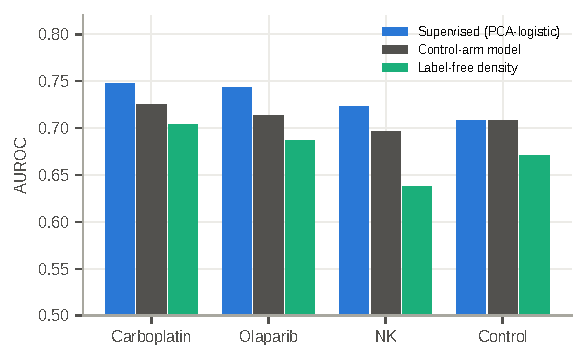
\includegraphics[width=\linewidth]{figures/FigS2_typicality.pdf}
  \caption*{\textbf{Supplementary Fig. 2 | Label-free typicality.} AUROC of the local-density score (negative mean distance to the 15 nearest neighbours within the sample), compared with the supervised PCA-logistic model and the control-arm (fitness) model, for each arm.}
\end{figure}


\begin{figure}[!htbp]
  \centering
  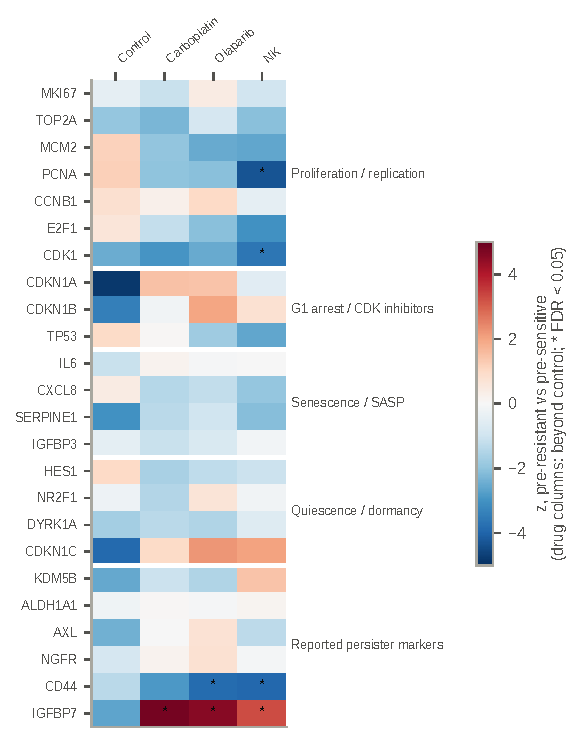
\includegraphics[width=\linewidth]{figures/FigS3_marker_panel.pdf}
  \caption*{\textbf{Supplementary Fig. 3 | Pre-specified marker panel.} z-scores for pre-resistant versus pre-sensitive cells. The control column shows the control (fitness) contrast; the drug columns show the difference from the control contrast, $z_{\text{diff}} = (z_{\text{drug}} - z_{\text{control}})/\sqrt{2}$. Asterisks mark FDR $<$ 0.05 for z\_diff. Genes not among the 5,005 retained genes (CDKN2A, RB1, GLB1, KDM5A) are omitted.}
\end{figure}


\begin{figure}[!htbp]
  \centering
  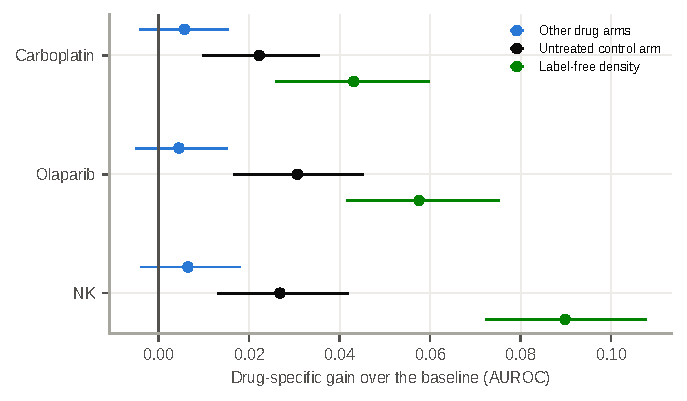
\includegraphics[width=\linewidth]{figures/FigS4_control_free.pdf}
  \caption*{\textbf{Supplementary Fig. 4 | Substitutes for an untreated arm.} For each drug arm of ReSisTrace, the drug-specific gain measured against the real control-arm model (black) and against two substitutes that use no control-arm labels: a model trained on the other drug arms (blue) and the label-free density score (green). Error bars are 95\% family-bootstrap intervals. The control-arm value lies between the two substitutes in every arm.}
\end{figure}


\begin{figure}[!htbp]
  \centering
  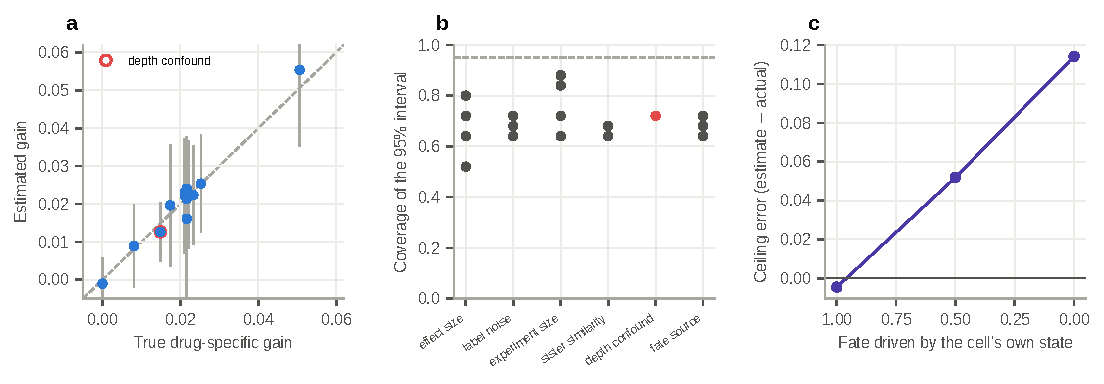
\includegraphics[width=\linewidth]{figures/FigS5_simulation.pdf}
  \caption*{\textbf{Supplementary Fig. 5 | The estimators checked against a known answer.} \textbf{a}, Estimated against true drug-specific gain across synthetic settings; the line is equality and bars are the spread over 25 independent experiments. \textbf{b}, Coverage of the nominal 95\% interval that resamples families without refitting the models, in each setting; the dashed line is 0.95. \textbf{c}, Estimated minus actual AUROC if the treated sister were scored, as fate moves from depending on the treated cell's own state (left, the estimator's assumption) to depending only on the state the sisters share (right).}
\end{figure}


\section*{References}

\noindent Chen T, Kornblith S, Norouzi M, Hinton G. A simple framework for contrastive learning of visual representations. \emph{ICML} (2020). arXiv:2002.05709\par\vspace{2pt}

\noindent Dai J, Zheng S, Falco MM, et al. Tracing back primed resistance in cancer via sister cells. \emph{Nat Commun} 15, 1158 (2024). doi:10.1038/s41467-024-45478-7 \par\vspace{2pt}

\noindent Hamilton WL, Ying R, Leskovec J. Inductive representation learning on large graphs. \emph{NeurIPS} (2017). arXiv:1706.02216\par\vspace{2pt}

\noindent Pellecchia S, Franchini M, Viscido G, et al. Single cell lineage tracing reveals clonal dynamics of anti-EGFR therapy resistance in triple negative breast cancer. \emph{Genome Med} 16, 55 (2024). doi:10.1186/s13073-024-01327-2 \par\vspace{2pt}

\noindent Schaff DL, White PE, Cote CJ, et al. Pre-existing cell states predict resistance to multiple treatments. \emph{Cell Genom} 6, 101191 (2026). doi:10.1016/j.xgen.2026.101191 \par\vspace{2pt}

\noindent Sharma SV, Lee DY, Li B, et al. A chromatin-mediated reversible drug-tolerant state in cancer cell subpopulations. \emph{Cell} 141, 69-80 (2010). doi:10.1016/j.cell.2010.02.027 \par\vspace{2pt}

\end{document}
